This chapter briefly introduces the basic concepts of physics engines. We restrict ourselves to the simulation of rigid bodies, which is a significant simplification of the problem since rigid bodies are idealized solid objects which never change shape.

\section{Problem statement}
We need to model the physical 

\section{Definitions}
A \textbf{mesh} is a 3D object made of vertices, edges and faces. 

A \textbf{convex mesh} is a mesh whose internal angles are all less or equal to $180\degree$.

\section{Kinematics}
The position of an object in a 3D space is given by a vector $p \in R^3$ from the origin of an inertial frame to the body fixed frame.

The orientation of an object in a 3D space can be represented in different ways. Usually it represented by either Euler angles or unit quaternions.

\section{Principles of rigid body dynamics simulation}
The section is heavily inspired by \cite{bender2014interactive}. The simulation of rigid body dynamics is usually built around the loop presented in \cref{fig:star_simul_loop}. The simulator begins by finding the collision points between objects (Collision detection). These points are used to derive motion laws which are solved to determine the forces that act on the objects and prevent them from inter-penetrating (Contact handling). Newly found contact points imply collisions, which generate infinite impulse forces, which are handled by collision resolution. When all the contact forces have been computed, the position and velocities of the bodies are integrated forward in time before a new iteration starts.

\begin{figure}[htp]
\center
\begin{subfigure}[b]{0.45\textwidth}
	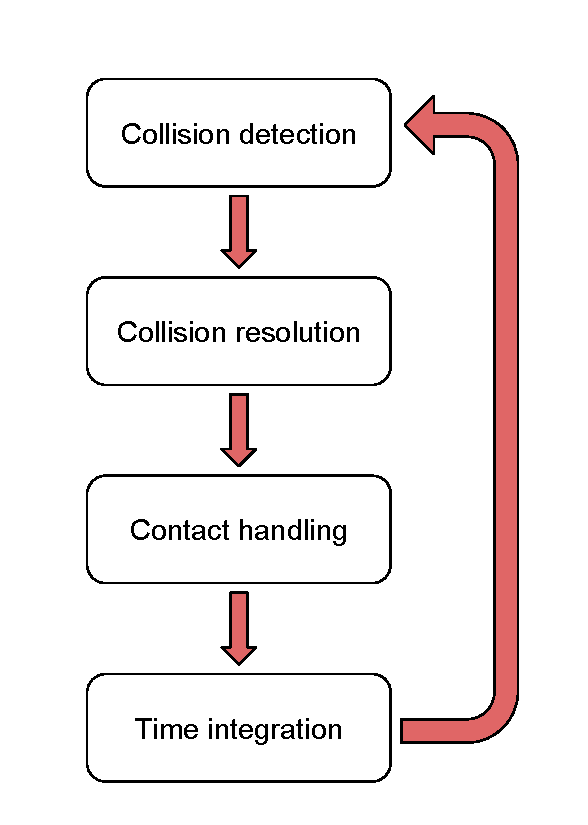
\includegraphics[width=\textwidth]{figures/star_simul_loop2}
	\caption[Simulation loop]{Modular description of the simulation loop of a physics engine}
	\label{fig:star_simul_loop}
\end{subfigure}
\hfill
\begin{subfigure}[b]{0.47\textwidth}
	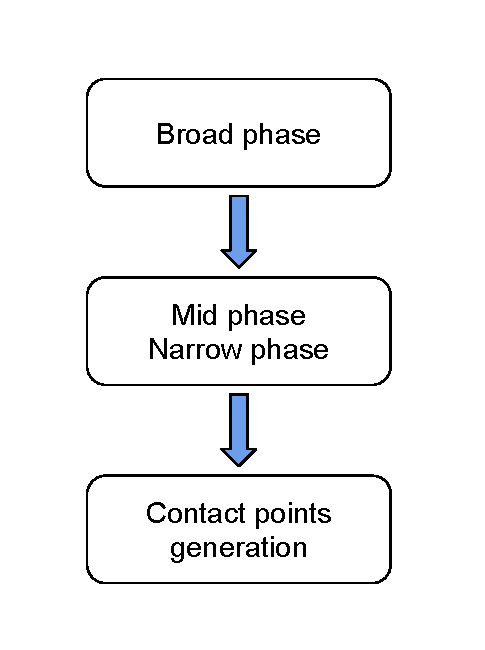
\includegraphics[width=\textwidth]{figures/STAR_collision}
	\caption[Collision detection]{Modular description of the collision detection in a physics engine.}
	\label{fig:star_collision}
\end{subfigure}
\caption[Modular phase description of the sub tasks of a rigid body simulator]{Modular phase description of the sub tasks of a rigid body simulator. The mid phase and narrow phase are grouped together because they are often combined for performance reasons}
\label{fig:phase_simul}
\end{figure}

\section{Collision detection}
Collision detect is broken into three phases called the broad phase, the mid phase and the narrow phase. 

During the broad phase, objects are approximated by simple geometric primitives. Distances between such geometric shapes are easy to compute. Spheres are usually used. If such spheres do not overlap, then neither do the actual objects.

When an object has a complex shape, an additional phase called the mid phase separates the object into several simpler shapes to detect collisions. Finally the narrow phase uses the exact geometries of the object to find the contact points. These are then returned to the simulation model.

\section{A quick primer}
Rigid body simulation is achieved through the expression of the Newton-Euler laws as differential equations which are then augmented with equations that express 3 conditions : nonpenetration of bodies, the friction model, and certain disjunctive relationships between variables (a contact force must become zero if two bodies separate, the friction forces acts in the direction that will most quickly stop the sliding).

This yields a differential nonlinear complementarity problem (dNCP) tha cannot be solved in closed form. It is discretized in time producing a series of NCPs whose solutions are an approximation of the state of the system.  This discrete solution is usually found by linearizing the NCP into a LCP to take advantage of the rich background for that type of problems.

\section{Newton-Euler}

